\section{Results}

\subsection{Clean accuracy is saturated}

Table~\ref{tab:sat} and Figure~\ref{fig:sat} report the four protocols over all eight models. Under the leakage-safe protocol seven of eight exceed 99.6\%, and the entire span is 2.5 points, from LeNet1D at 0.975 to MCNN at 1.000. The heat map makes the point visually: the two leftmost columns are a single colour.

Changing the split, by contrast, moves everything. The cross-load protocol costs 5 to 13 points per model (WDCNN 0.948, LeNet1D 0.856), i.e.\ 10 points on average, and it is the only column with visible structure. WDCNN is the best model there although it is only fifth under the leakage-safe protocol; the three narrow-kernel convolutional backbones (MCNN, ResNet1D, DS-CNN) all land within half a point of 0.899, which we read as a ceiling of the 10-class task across loads rather than as a property of the three models. The recording-disjoint column sits in between and carries the largest seed spread (WDCNN $0.955\pm0.052$), so we treat it as a consistency check rather than a ranking.

Leakage is a small effect. Leaky is above safe for all eight models, but by at most 0.63 points (LeNet1D 0.982 vs.\ 0.975) and by 0.3 points or less for seven of them---an order of magnitude below what recent critiques of vibration benchmarks imply~\citep{phme2026,ssrn2024}. The protocol choice (leaky $\rightarrow$ cross-load) costs 5--13 points, i.e.\ 20 to 40 times more than leakage. The same comparison in a 20-windows-per-class regime, where the overlap removes a much larger fraction of the training windows, gives a mean leaky-minus-safe gap of $+0.4$ points (four models, two seeds, at most $+0.9$ for WDCNN); that regime reduces accuracy from 0.38 (LeNet1D) to 0.98 (MCNN) and thus exposes model differences that full data hides, but leakage remains negligible there too.

\textbf{Finding 1.} Every lightweight model reaches $\geq 97.5\%$ under a leakage-safe protocol. The benchmark is saturated: the eight models span 2.5 points, less than the effect of changing the split, so clean CWRU accuracy cannot rank architectures or support the architectural claims in the literature.

\textbf{Finding 2.} Overlapping-window leakage inflates accuracy by at most 0.6 points at full data and by at most 0.9 points in a 20-windows-per-class regime. The contamination of the CWRU literature comes from the split protocol, not from leakage, and the more serious problem is saturation.

\begin{table}[t]
\centering
\caption{Clean test accuracy (mean$\pm$std over two seeds, 20 epochs, 10-class CWRU) under four split protocols. \emph{leaky}: random window-level split with 50\% overlap between neighbouring windows; \emph{safe}: recording-level split with a $w/2$ guard band and zero shared sampling points; \emph{cross-load}: train on loads 0--2, test on load 3; \emph{recording-disjoint}: train and test on disjoint recordings. Best value per column in bold; columns whose maximum is shared by several models are left unbolded.}
\label{tab:sat}
\begin{tabular}{lcccc}
\toprule
model & leaky & safe & cross-load & recording-disjoint\\
\midrule
WDCNN        & .999$\pm$.000 & .997$\pm$.001 & \best{.948}$\pm$.003 & .955$\pm$.052\\
TICNN        & 1.000$\pm$.000 & 1.000$\pm$.000 & .911$\pm$.013 & .997$\pm$.005\\
MCNN         & 1.000$\pm$.000 & 1.000$\pm$.000 & .900$\pm$.000 & .997$\pm$.004\\
ResNet1D     & 1.000$\pm$.000 & 1.000$\pm$.000 & .899$\pm$.000 & .997$\pm$.002\\
DS-CNN       & 1.000$\pm$.000 & 1.000$\pm$.000 & .900$\pm$.001 & \best{.998}$\pm$.003\\
LeNet1D      & .982$\pm$.003 & .975$\pm$.002 & .856$\pm$.002 & .954$\pm$.048\\
ViT1D        & .998$\pm$.001 & .996$\pm$.002 & .894$\pm$.009 & .986$\pm$.012\\
MLP-Mixer1D  & .999$\pm$.001 & .996$\pm$.001 & .870$\pm$.008 & .953$\pm$.050\\
\midrule
spread & 1.8 & 2.5 & 9.1 & 4.5\\
\bottomrule
\end{tabular}
\end{table}

\begin{figure}[t]
\centering
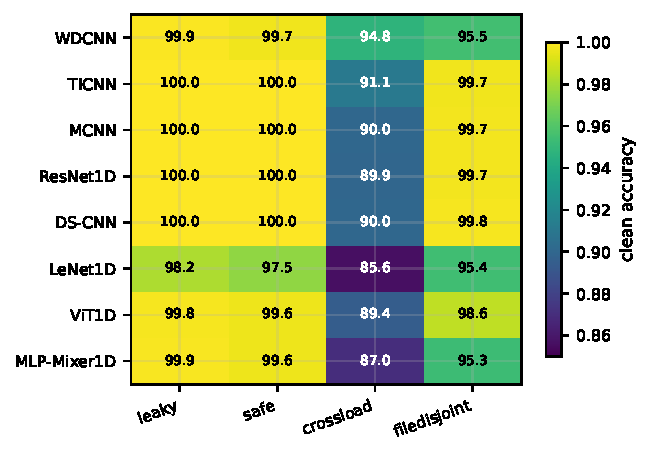
\includegraphics[width=.62\textwidth]{../figures/fig1_saturation.pdf}
\caption{Clean test accuracy of eight lightweight models under four split protocols. Overlapping-window leakage (leftmost column) and the leakage-safe protocol are indistinguishable; the cross-load column is the only one that separates models.}
\label{fig:sat}
\end{figure}

\subsection{Noise stress: a 55-point spread and a rank inversion}

Table~\ref{tab:e2} reports the same models evaluated on noisy test signals. The clean column is uninformative: the 10\,dB column spans \best{0.427 to 0.980}, i.e.\ 55 points.

\textbf{Finding 3.} At 10\,dB SNR the eight architectures are separated by 55 points, while on clean data they are separated by 3. Three models above 99.5\% clean accuracy fall below 60\% at 10\,dB. Across the eight models, the Spearman correlation between clean and 10\,dB accuracy is $\rho=-0.38$ ($p=0.35$, $n=8$): not merely uninformative but slightly negative. The only architectures that survive are the two with wide first-layer kernels (WDCNN, TICNN).

\begin{table*}[t]
\centering
\caption{Clean-trained models, test accuracy (mean over 3 seeds) at six SNRs. “Clean” is the uncorrupted test set. Standard deviations at 10\,dB are given in parentheses; the highest and the lowest 10\,dB entry are bold. The full per-seed table accompanies the released results.}
\label{tab:e2}
\begin{tabular}{lrrrrrrr}
\toprule
model & params & clean & 15\,dB & 10\,dB & 5\,dB & 0\,dB & $-5$\,dB\\
\midrule
WDCNN       & 34{,}410  & .9970 & .9953 & \best{.9803} (.010) & .8362 & .4053 & .1310\\
TICNN       & 83{,}914  & .9998 & .9998 & .9571 (.019) & .6465 & .2887 & .1377\\
ViT1D       & 139{,}850 & .9964 & .9741 & .7553 (.005) & .4675 & .2705 & .1294\\
MLP-Mixer1D & 747{,}722 & .9968 & .9772 & .7504 (.019) & .4433 & .3051 & .1999\\
LeNet1D     & 3{,}018   & .9698 & .9470 & .7062 (.075) & .4080 & .1690 & .1067\\
MCNN        & 184{,}554 & 1.0000& .9315 & .5856 (.038) & .2507 & .1004 & .1005\\
DS-CNN      & 69{,}642  & .9995 & .7887 & .4281 (.016) & .2969 & .2281 & .1296\\
ResNet1D    & 241{,}322 & .9999 & .8051 & \best{.4271} (.012) & .2646 & .1357 & .1294\\
\bottomrule
\end{tabular}
\end{table*}

\begin{figure*}[t]
\centering
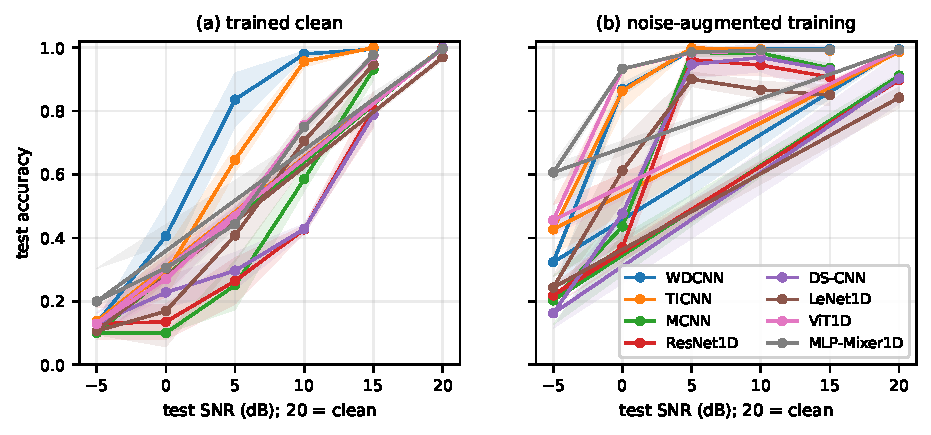
\includegraphics[width=\textwidth]{../figures/fig2_noise.pdf}
\caption{Test accuracy versus SNR for the eight architectures. (a) Trained on clean data: at 10\,dB the models span 55 points and the ordering is unrelated to clean accuracy. (b) Trained with per-batch noise augmentation: at 10\,dB the curves collapse into a band of 0.87--1.00, i.e.\ from a 55-point spread to 13 points. Shaded regions are $\pm1$ std over three seeds.}
\label{fig:noise}
\end{figure*}

\subsection{Noise augmentation repairs most of the gap}

Table~\ref{tab:e4} repeats the matrix with one change: during training, each mini-batch draws a random SNR from $U[0,15]$\,dB.

\textbf{Finding 4.} Augmentation compresses the 10\,dB spread from 55 to 13 points and lifts the worst clean-trained model at 10\,dB (DS-CNN) from 43\% to 95\%, and even the weakest augmented model reaches 87\%. Averaged over the 24 (model, seed) pairs, 10\,dB accuracy rises from .699 to .967 ($+26.8$ points, Holm-corrected $p<10^{-6}$), 5\,dB from .452 to .970 and 0\,dB from .238 to .687 (Table~\ref{tab:wilcoxon}). The price is 5.4 points of clean accuracy, concentrated in the small and deep models; the two wide-kernel models lose at most 2 points. This is a better trade than any architectural change we tried.

\begin{table*}[t]
\centering
\caption{As Table~\ref{tab:e2}, but with noise augmentation (SNR $\sim U[0,15]$\,dB per mini-batch) during training.}
\label{tab:e4}
\begin{tabular}{lrrrrrr}
\toprule
model & clean & 15\,dB & 10\,dB & 5\,dB & 0\,dB & $-5$\,dB\\
\midrule
WDCNN       & .9949 & .9953 & \best{.9953} & .9927 & .8697 & .3236\\
TICNN       & .9872 & .9909 & .9951 & .9991 & .8638 & .4271\\
ViT1D       & .9933 & .9924 & .9904 & .9840 & .9333 & .4557\\
MLP-Mixer1D & .9938 & .9930 & .9920 & .9854 & .9335 & .6066\\
MCNN        & .9121 & .9357 & .9831 & .9846 & .4362 & .2032\\
DS-CNN      & .9029 & .9299 & .9693 & .9471 & .4772 & .1624\\
ResNet1D    & .8975 & .9073 & .9450 & .9623 & .3704 & .2188\\
LeNet1D     & .8428 & .8505 & \worst{.8672} & .9005 & .6124 & .2437\\
\bottomrule
\end{tabular}
\end{table*}

\begin{table}[t]
\centering
\caption{Paired Wilcoxon signed-rank tests, clean-trained vs.\ augmented, pairs = model $\times$ seed ($n=24$), Holm-corrected.}
\label{tab:wilcoxon}
\begin{tabular}{lrrrr}
\toprule
metric & clean-trained & +aug & $\Delta$ & $p_{\text{Holm}}$\\
\midrule
clean     & .9949 & .9405 & $-0.0543$ & $3.6\times10^{-5}$\\
10\,dB    & .6988 & .9672 & $+0.2684$ & $4.8\times10^{-7}$\\
5\,dB     & .4517 & .9695 & $+0.5178$ & $3.6\times10^{-5}$\\
0\,dB     & .2379 & .6871 & $+0.4492$ & $4.8\times10^{-7}$\\
\bottomrule
\end{tabular}
\end{table}

\begin{figure*}[t]
\centering
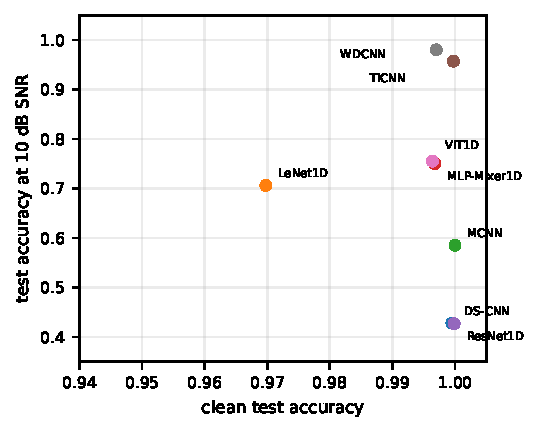
\includegraphics[width=0.62\textwidth]{../figures/fig3_rank_inversion.pdf}
\hfill
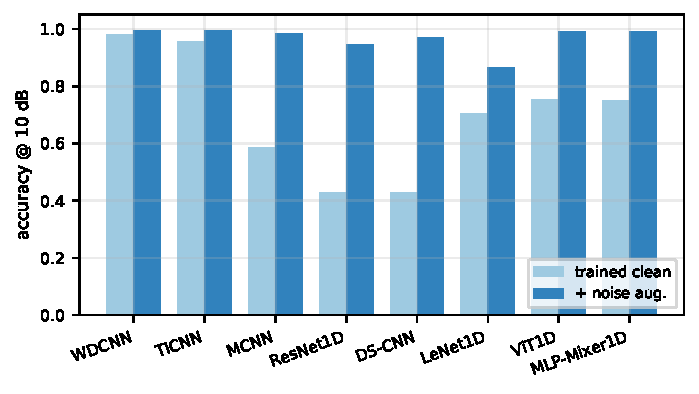
\includegraphics[width=0.34\textwidth]{../figures/fig4_aug_gain.pdf}
\caption{Left: clean accuracy versus 10\,dB accuracy for the eight models trained on clean data. The ordering is not preserved and the point cloud slopes the wrong way. Right: augmentation closes the 10\,dB gap for every model.}
\label{fig:rank}
\end{figure*}

\subsection{A multi-channel front-end buys robustness almost for free}

The previous two subsections suggest that robustness lives in what happens at the input: noise augmentation changes the input distribution during training, and wide first-layer kernels act as a fixed band-pass. To test the second mechanism directly we insert a learnable front-end---$c$ parallel convolutions with kernel $k$ and stride $s$, concatenated in the channel dimension---in front of narrow-kernel backbones, and sweep $(k,c)\in\{(32,8),(64,1),(64,4),(64,8),(128,8)\}$ (Table~\ref{tab:stem}).

\textbf{Finding 5.} The number of front-end channels, not the kernel width, is the decisive knob. For ResNet1D, one wide channel ($k=64,c=1$) buys $+34.3$ points at 10\,dB but costs 12.7 clean points; $c=8$ at the same $k$ buys $+49.6$ points for only 0.7 clean points; widening to $k=128$ adds another 2.7 points at 10\,dB for 512 more parameters, i.e.\ a 25\% larger front end. A multi-channel wide stem is therefore the cheapest single change a practitioner can make to a narrow-kernel backbone: 2{,}608 parameters, or 1.1\% of the ResNet1D backbone. The gain is largest where the backbone is most brittle ($+49.6$ for ResNet1D, $+49.8$ for DS-CNN) and smallest where the backbone already mixes the whole window ($+13.3$ for ViT1D).

\begin{table}[t]
\centering
\caption{Wide-kernel front-end ablation (clean training, noise only at test time, one seed, 15 epochs). $\Delta$ relative to the same backbone without a front-end.}
\label{tab:stem}
\begin{tabular}{lrrrrrr}
\toprule
config & params & clean & 10\,dB & 5\,dB & 0\,dB & $\Delta$10\,dB\\
\midrule
ResNet1D plain          & 241{,}322 & 1.0000 & .4534 & .2060 & .1000 & 0\\
ResNet1D $k64c1$        & 241{,}388 & .8728 & .7959 & .6463 & .3690 & $+34.3$\\
ResNet1D $k64c4$        & 242{,}258 & .9739 & .9231 & .7907 & .4556 & $+47.0$\\
ResNet1D $k64c8$        & 243{,}418 & .9929 & .9496 & .7910 & .3955 & $+49.6$\\
ResNet1D $k32c8$        & 243{,}162 & .9918 & .8799 & .5619 & .3433 & $+42.7$\\
ResNet1D $k128c8$       & 243{,}930 & .9854 & \best{.9765} & .8799 & .4966 & $+52.3$\\
DS-CNN plain            & 69{,}642 & .9996 & .4224 & .2780 & .2131 & 0\\
DS-CNN $k64c8$          & 71{,}290 & .9799 & .9201 & .5896 & .2224 & $+49.8$\\
MCNN plain              & 184{,}554 & 1.0000 & .5974 & .3097 & .1011 & 0\\
MCNN $k64c8$            & 185{,}418 & .9948 & .9884 & \best{.9332} & \best{.5343} & $+39.1$\\
ViT1D plain             & 139{,}850 & .9963 & .7720 & .4858 & .2127 & 0\\
ViT1D $k64c8$           & 143{,}706 & .9918 & .9049 & .7474 & .3489 & $+13.3$\\
\bottomrule
\end{tabular}
\end{table}

\begin{figure}[t]
\centering
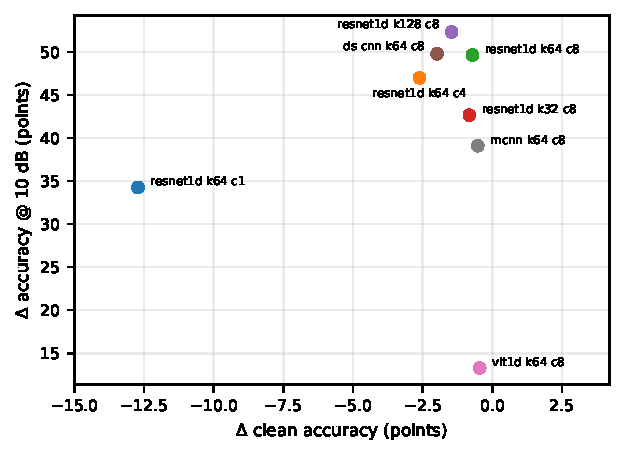
\includegraphics[width=0.62\textwidth]{../figures/fig5_stem_tradeoff.pdf}
\caption{Trade-off of the wide multi-channel front-end: change in 10\,dB accuracy against change in clean accuracy, relative to the same backbone without a stem. Configurations in the lower-right quadrant are strictly dominated.}
\label{fig:stem}
\end{figure}

\subsection{The two mechanisms compose, and the front-end makes augmentation cheap}
\label{sec:combo}

The two interventions act on different parts of the pipeline, so they need not be alternatives. Table~\ref{tab:combo} crosses them: for the four most brittle backbones, we train with neither, with augmentation only, with a stem only, and with both (stem $k64c8$, and $k128c8$ for ResNet1D; three seeds, 20 epochs).

\textbf{Finding 6.} The combination is the best configuration at 10\,dB for three of the four backbones (ResNet1D 0.989, DS-CNN 0.973, MCNN 0.995) and ties for best in the fourth (ViT1D 0.978 vs.\ 0.991 for augmentation alone). Two effects make it strictly preferable to either intervention alone. First, the front-end cancels most of the clean-accuracy cost of augmentation: augmentation alone costs 0.3--15 clean points on these backbones, while stem plus augmentation costs 0.6--4.3, because the parallel band-pass filters absorb the distribution shift that the noise schedule introduces. Second, the largest gains appear at low SNR: at 0\,dB, moving from plain to stem plus augmentation adds 73, 49, 81 and 61 points respectively, and even at $-5$\,dB (outside the augmentation range) the gain remains 11--43 points.

ViT1D is the exception that confirms the mechanism: its patch embedding already performs a learned projection of the whole window, so the front-end adds only 15 points at 10\,dB, less than the 24 points of pure augmentation. For ViT-style backbones the recipe, not the input layer, is the lever.

\begin{table}[t]
\centering
\caption{Four-quadrant comparison of the front-end and noise augmentation (clean training vs.\ SNR $\sim U[0,15]$ per batch; three seeds). $\Delta$ in points relative to the plain backbone.}
\label{tab:combo}
\begin{tabular}{llrrrrr}
\toprule
model & condition & clean & 10\,dB & 5\,dB & 0\,dB & $\Delta$clean / $\Delta$10\,dB \\
\midrule
ResNet1D & plain    & 1.000 & .427 & .265 & .136 & --- \\
         & +aug     & .889  & .917 & .996 & .428 & $-11.1$ / $+49.0$ \\
         & stem     & .989  & .973 & .840 & .463 & $-1.1$ / $+54.6$ \\
         & stem+aug & .986  & \best{.989} & .987 & .865 & $-1.4$ / $+56.2$ \\
\addlinespace
DS-CNN   & plain    & 1.000 & .428 & .297 & .228 & --- \\
         & +aug     & .853  & .944 & .993 & .481 & $-14.6$ / $+51.6$ \\
         & stem     & .974  & .931 & .699 & .269 & $-2.6$ / $+50.3$ \\
         & stem+aug & .957  & \best{.973} & .976 & .716 & $-4.3$ / $+54.4$ \\
\addlinespace
MCNN     & plain    & 1.000 & .586 & .251 & .100 & --- \\
         & +aug     & .920  & .980 & .982 & .419 & $-8.0$ / $+39.5$ \\
         & stem     & .995  & .989 & .933 & .488 & $-0.6$ / $+40.3$ \\
         & stem+aug & .994  & \best{.995} & .992 & \best{.911} & $-0.6$ / $+41.0$ \\
\addlinespace
ViT1D    & plain    & .996  & .755 & .468 & .271 & --- \\
         & +aug     & .994  & \best{.991} & .983 & \best{.935} & $-0.3$ / $+23.6$ \\
         & stem     & .992  & .905 & .712 & .358 & $-0.5$ / $+14.9$ \\
         & stem+aug & .976  & .978 & .976 & .885 & $-2.0$ / $+22.3$ \\
\bottomrule
\end{tabular}
\end{table}

